\documentclass[
  captions=tableheading,
  bibliography=totoc, 
  titepage=firstiscover,
]{scrartcl}

\usepackage{blindtext} %neuer input

\usepackage{longtable} % Tabellen über mehrere Seiten

\usepackage[utf8]{inputenc} %neuer input

\usepackage{scrhack}

\usepackage[aux]{rerunfilecheck} %Warnung falls nochmal kompiliert werden muss

\usepackage{fontspec} %Fonteinstellungen

\recalctypearea{}

\usepackage[main=ngerman]{babel} %deutsche Spracheinstellung

\usepackage{ragged2e} %neuer input

\usepackage{amsmath, nccmath}

\usepackage{amssymb} %viele mathe Symbole

\usepackage{mathtools} %Erweiterungen für amsmath


\DeclarePairedDelimiter{\abs}{\lvert}{\rvert}
\DeclarePairedDelimiter{\norm}{\lVert}{\rVert}

\DeclarePairedDelimiter{\bra}{\langle}{\rvert}
\DeclarePairedDelimiter{\ket}{\lvert}{\rangle}

\DeclarePairedDelimiterX{\braket}[2]{\langle}{\rangle}{
#1 \delimsize| #2
}

\NewDocumentCommand \dif {m}
{
\mathinner{\symup{d} #1}
}


\usepackage[
  math-style=ISO,
  bold-style=ISO,
  sans-style=italic,
  nabla=upright,
  partial=upright,
  warnings-off={
    mathtools-colon,
    mathtools-overbracket,
  },
]{unicode-math}

\setmathfont{Latin Modern Math}
\setmathfont{XITS Math}[range={scr, bfscr}]
\setmathfont{XITS Math}[range={cal, bfcal}, StylisticSet=1]


\usepackage[
  locale=DE,
  separate-uncertainty=true,
  per-mode=reciprocal,
  output-decimal-marker={,},
]{siunitx}

\usepackage[autostyle]{csquotes} %richtige Anführungszeichen

\usepackage{xfrac}

\usepackage{float}

\floatplacement{figure}{htbp}

\floatplacement{table}{htbp}

\usepackage[ %floats innerhalb einer section halten
  section,   %floats innerhalb er section halten
  below,     %unterhalb der Section aber auf der selben Seite ist ok
]{placeins}

\usepackage[
  labelfont=bf,
  font=small,
  width=0.9\textwidth,
]{caption}

\usepackage{subcaption} %subfigure, subtable, subref

\usepackage{graphicx}

\usepackage{grffile}

\usepackage{booktabs}

\usepackage{microtype} %Verbesserungen am Schriftbild

\usepackage[
backend=biber,
]{biblatex}

\addbibresource{../lit.bib}

\usepackage[ %Hyperlinks im Dokument
  german,
  unicode,
  pdfusetitle,
  pdfcreator={},
  pdfproducer={},
]{hyperref}

\usepackage{bookmark}

\usepackage[shortcuts]{extdash}

%\usepackage{warpcol}

\graphicspath{ {./V802/} }  % der path zum Ordner mit den Bildern funktioniert ähnlich wie beim Input command
\begin{document}
    \title{V802 Fouriersynthese}
    \author{  
    Tobias Rücker\\
    \texorpdfstring{\href{mailto:tobias.ruecker@tu-dortmund.de}{tobias.ruecker@tu-dortmund.de}
    \and}{,} 
    Paul Störbrock\\
    \texorpdfstring{\href{mailto:paul.stoerbrock@tu-dortmund.de}{paul.stoerbrock@tu-dortmund.de}}{}
    }
    \date{Durchführung: 14.11.2019, Abgabe: 19.11.2019\vspace{-4ex}}
\maketitle
\center{\Large Versuchsgruppe: \textbf{42}}
    
    \begin{abstract}
        \textbf{Ziel:} Bestimmung der Fourierkoeffizienten und Darstellung der Fouriersynthese 
    \end{abstract}
    
\newpage
\justifying

\section{Versuchsauswertung:}

    

    \begin{align}   % align Umgebung sieht schmucker aus als die equation Umgebung
        &f(t) = \sum_{k=0}^{\infty} (A_k \cos(\omega_kt) + B_k \sin(w_kt))  &\text{mit} \:\: \omega_k = \frac{2\pi k}{T} \label{eq:frow}\\
        &A_k \hphantom{)} = \frac{2}{T} \int_{-T/2}^{+T/2} f(t) \cos(\omega_kt) dt  &\text{mit} \:\: A_0 = \frac{1}{T} \int f(t)dt \label{eq:Ak}\\
        &B_k \hphantom{)} = \frac{2}{T} \int_{-T/2}^{+T/2} f(t) \sin(w_kt) dt \!\!&\text{mit} \:\: B_0 = 0 \label{eq:Bk}
    \end{align}
    Mithilfe der Formeln \eqref{eq:Ak} und \eqref{eq:Bk} erhalten wir durch Einsetzen der gegebenen Funktion
    \begin{align}
        f(t) = \abs{\sin(t)} \label{eq:abs_sin} 
    \end{align}
    die folgenden Fourierkoeffizienten für $A_k$ und $B_k$:
    \begin{align*}
        &A_0 = \frac{2}{\pi} &A_k = -\frac{4}{\pi}\:\frac{1}{4k^{2}-1}\\
        &B_0 = 0 &B_k = 0
    \end{align*}
    damit sieht die Fourierreihe für \eqref{eq:abs_sin} folgendermaßen aus:
    \begin{align}
        f(t)=\frac{2}{\pi}+\sum_{k=1}^{\infty} \left(-\frac{4}{\pi} \:\frac{1}{4k^2+1} \cos(2kt)\right)
    \end{align}
    \begin{figure}[h]
         \centering
         \fbox{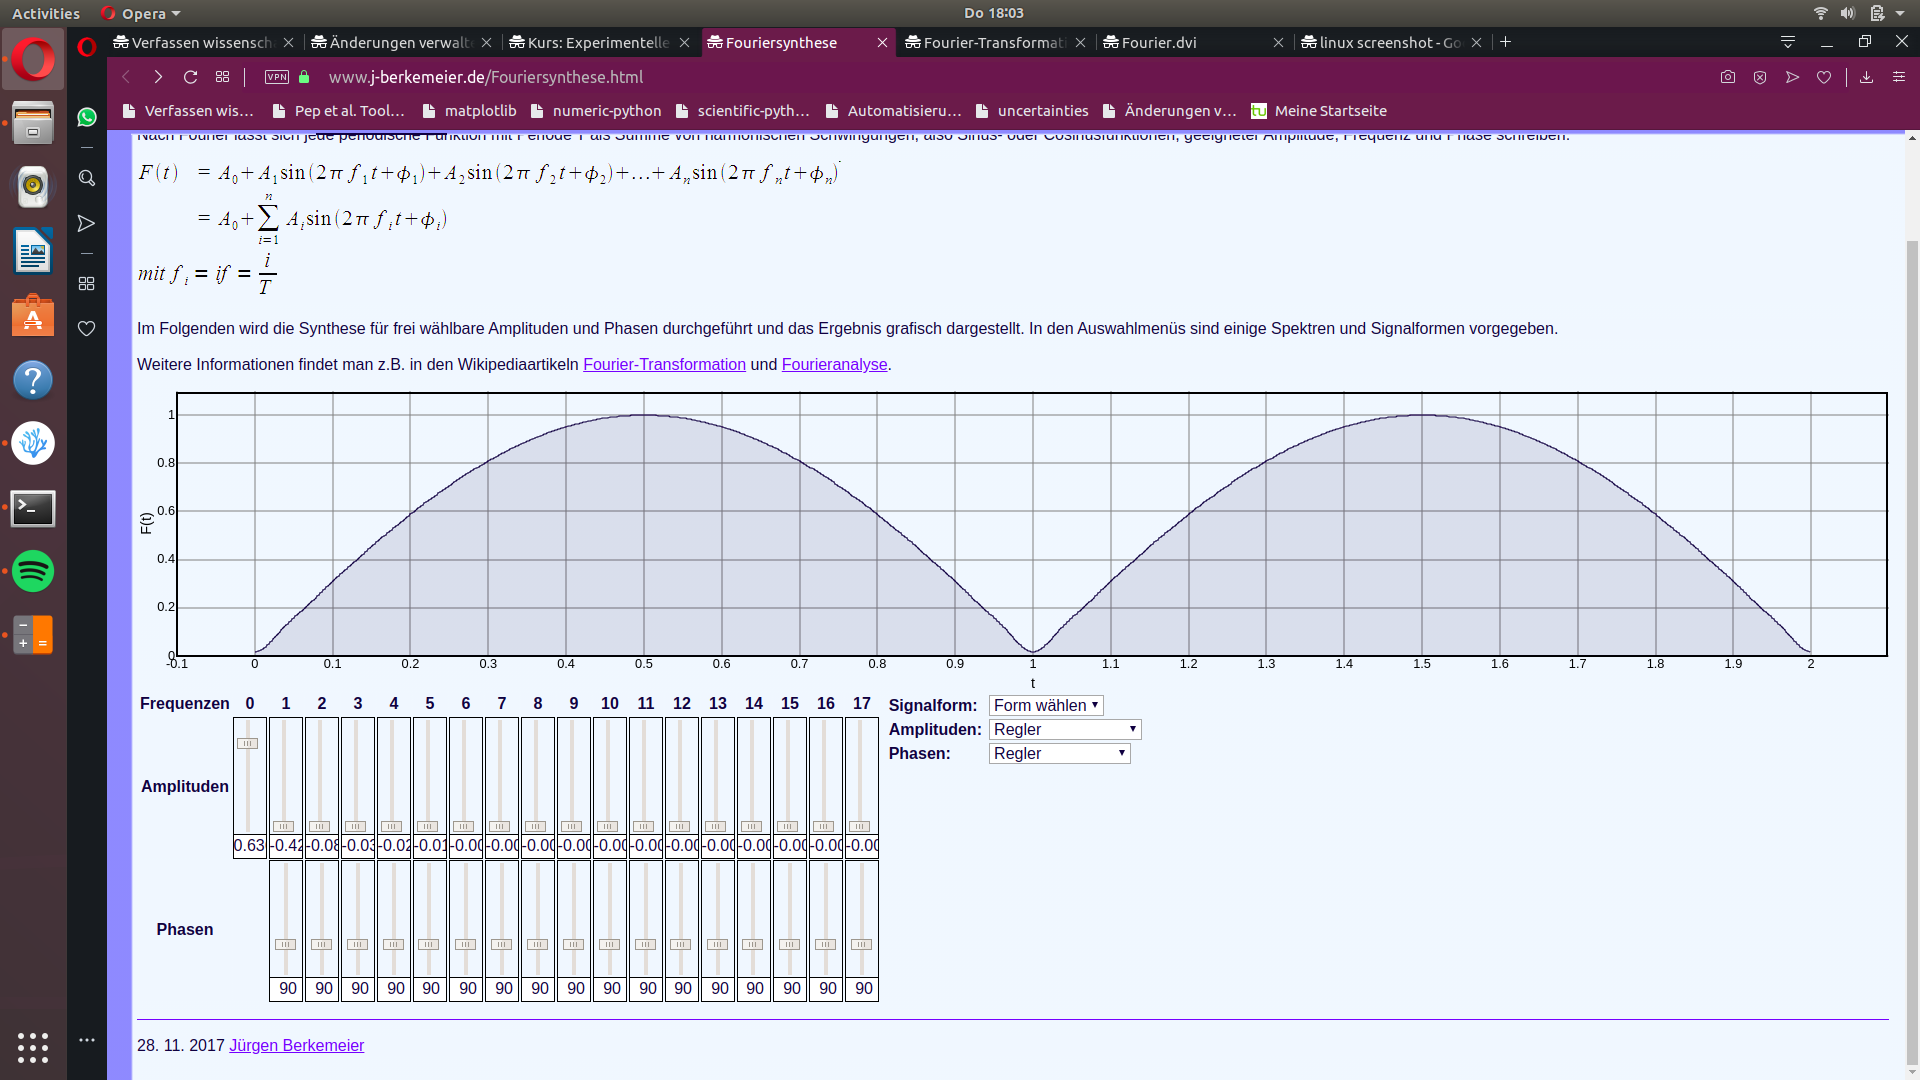
\includegraphics[width=\textwidth]{abs_sinx_fourier}}  \vspace{-1.5em}
         \caption{Darstellung der Fourierreihe von der Funktion \eqref{eq:abs_sin}}
         \label{fig:sc_sin} 
    \end{figure}
    \newpage
    Mit der zweiten Funktion
    \begin{align}
        &f(t) = t &\text{für} -\pi < x < \pi \label{eq:t}
    \end{align}
    erhalten wir die folgenden Koeffizienten für $A_k$ und $B_k$:
    \begin{align*}
        &A_0 = 0 &A_k &= 0\\
        &B_0 = 0 &B_k &= \frac{2}{k}\:(-1)^{k+1}
    \end{align*}
    Die Fourierreihe für \eqref{eq:t} sieht damit folgendermaßen aus:

    \begin{align}
        f(t)= \sum_{k=1}^{\infty} \left(\frac{2}{k} (-1)^{k+1}\right)
    \end{align}
    \begin{figure}[h]   % Screenshot für Darstellung der Fourierreihe von f(t) = t
        \centering
        \fbox{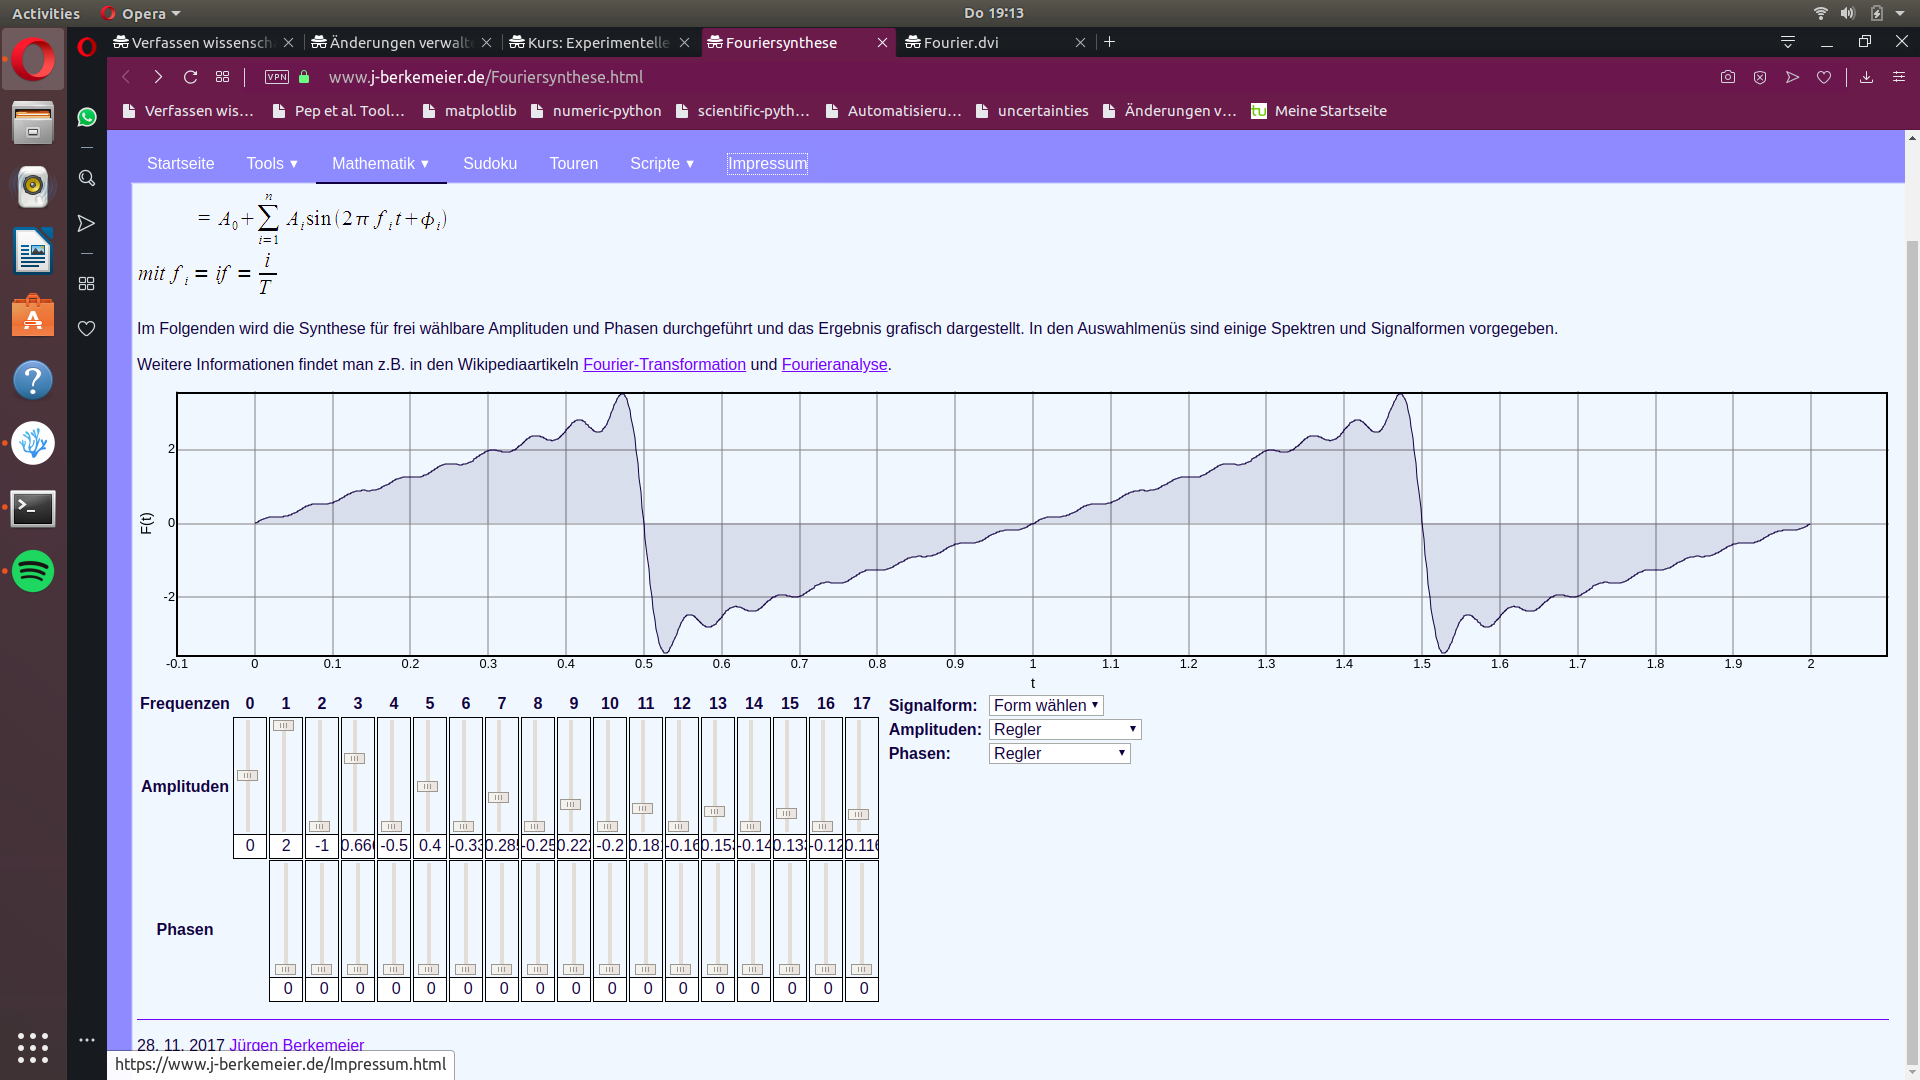
\includegraphics[width=\textwidth]{x_fourier}}
        \caption{Darstellung der Fourierreihe von der Funktion \eqref{eq:t}} \vspace{-1.5em}
        \label{fig:sc_t}
    \end{figure}

\end{document}